\documentclass{article}
\usepackage[utf8]{inputenc}
\usepackage{graphicx}
\setlength{\parindent}{0pt}
\setlength{\parskip}{1em}

\title{FOAR705 - Learning Journal Week 5 - Software Carpentry Exercises}
\author{Jan Jugueta - 44828020}
\date{Week 5: 23/8/19 - 29/8/19}

\begin{document}

\maketitle

\section*{28/8/19 - 2:15pm}

Beginning the exercises in Software Carpentry. Some key points in the \textbf{Introducing the Shell} lesson.

\begin{itemize}
    \item There are different ways to interact with a computer:
    \begin{itemize}
        \item Graphical user interface (GUI) which normally uses a mouse.
        \item Command-line interface which requires the knowledge of commands.
    \end{itemize}
    \item The Shell is a program which runs other programs than doing calculations itself.
    \item The shell's main advantages are its high action-to-keystroke ratio, its support for automating repetive tasks, and its capacity to access networked machines.
    \item The shell's main disadvantages are its primarily textual nature and how cryptic its command and operation can be.
\end{itemize}

\section*{28/8/19 - 2:32pm}

Continuing on with the next lesson \textbf{Navigating Files and Directories}. Below are some useful commands.

\begin{verbatim}
    pwd (Tells us which directory we are in)
    ls (Gives a listing in the directory)
    -F (Is a switch or a flag)
    man ls (Brings up a manual)
\end{verbatim} 

\section*{28/8/19 - 3:03pm}

Below is the exercise \textit{Exploring More ls Flags}

\textbf{Objective:} See what happens when I use both the -l and -h option.

\textbf{Action:}
\begin{itemize}
    \item Entered the command \begin{verbatim}
        ls -l
    \end{verbatim}
    \item Entered the command \begin{verbatim}
        ls -l -h
    \end{verbatim}
    \item Entered the command \begin{verbatim}
        ls -h
    \end{verbatim}
\end{itemize}

\textbf{Error:} None.

\textbf{Result:} The -l command makes the listing a long format. The -h and -l option makes it more readable for a human.

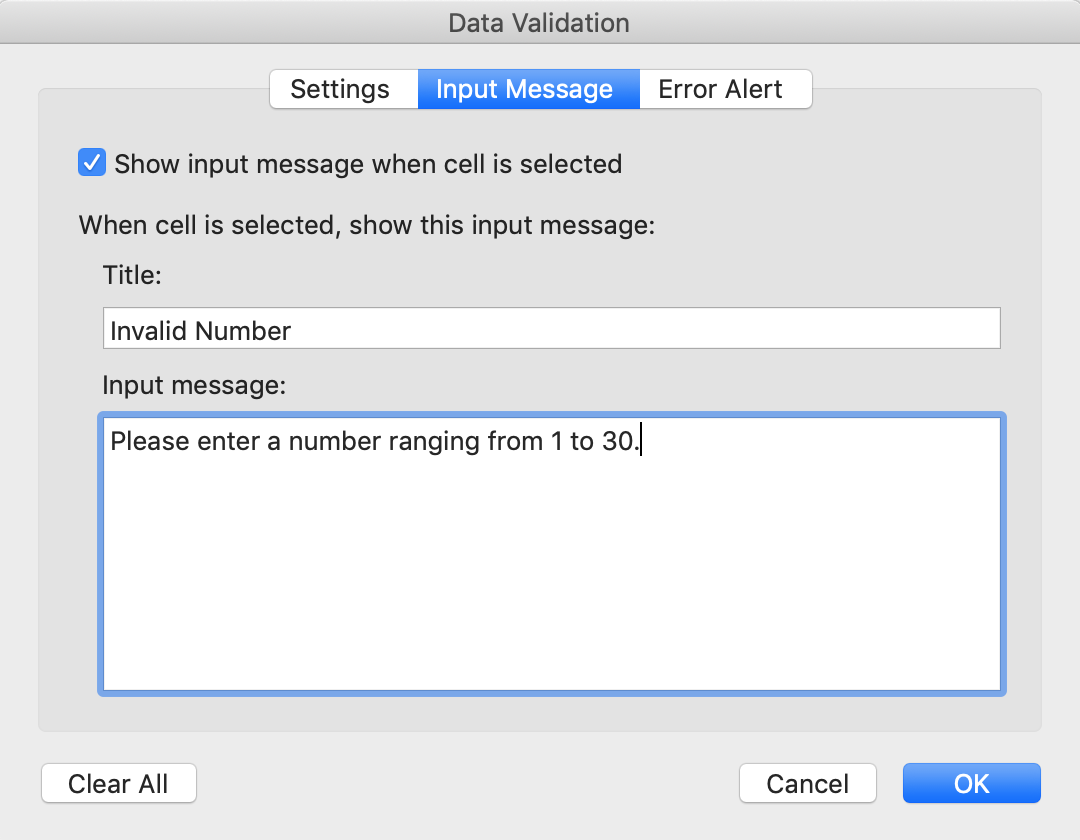
\includegraphics[width=\textwidth]{figa.png}

\section*{28/8/19 - 3:10pm}

Continuing on with the exercise \textit{Listing Recursively and By Time}

\textbf{Objective:} Find out what order ls -R -t displays things.

\textbf{Action:} Entered the command \begin{verbatim}
    ls -R -t
\end{verbatim}

\textbf{Error:} None.

\textbf{Result:} Not sure what quite happened but it did list ALOT of things. The solution on Software Carpentry says that it sorts it by time of last change.

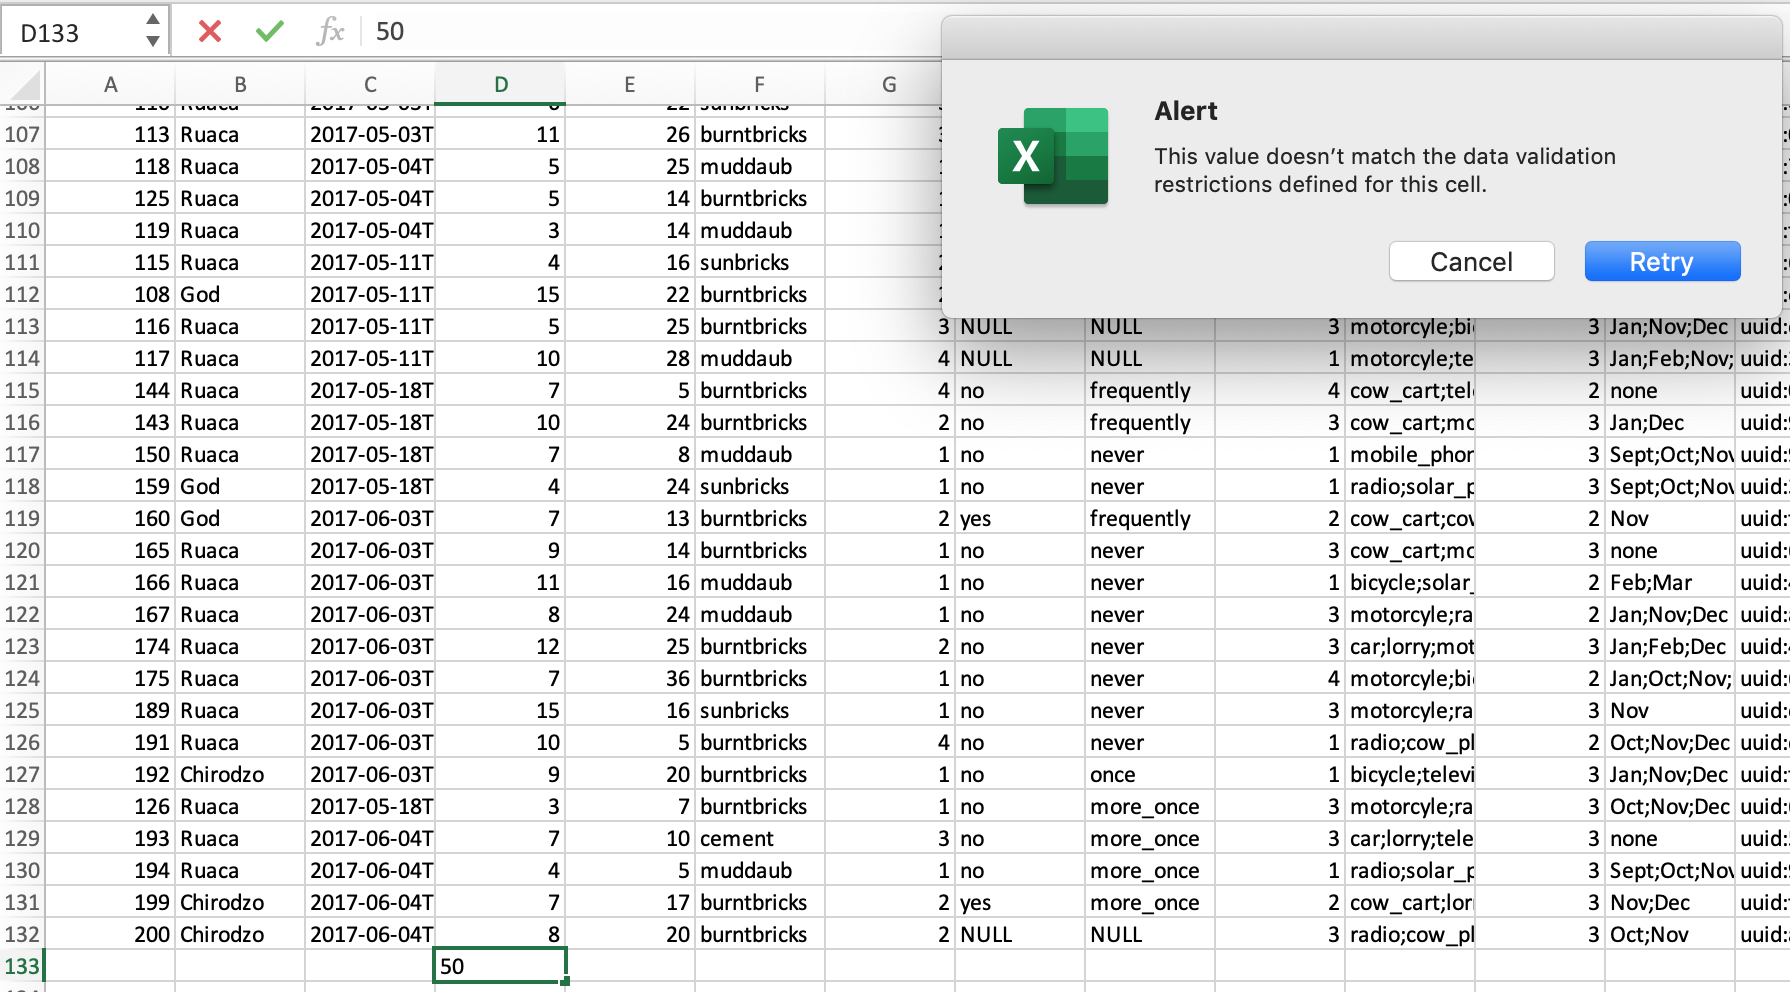
\includegraphics[width=\textwidth]{figb.png}

\section*{28/8/19 - 3:24pm}

Have kept on following the instructions of the lesson and the only problem that I have encountered a typo error I entered.

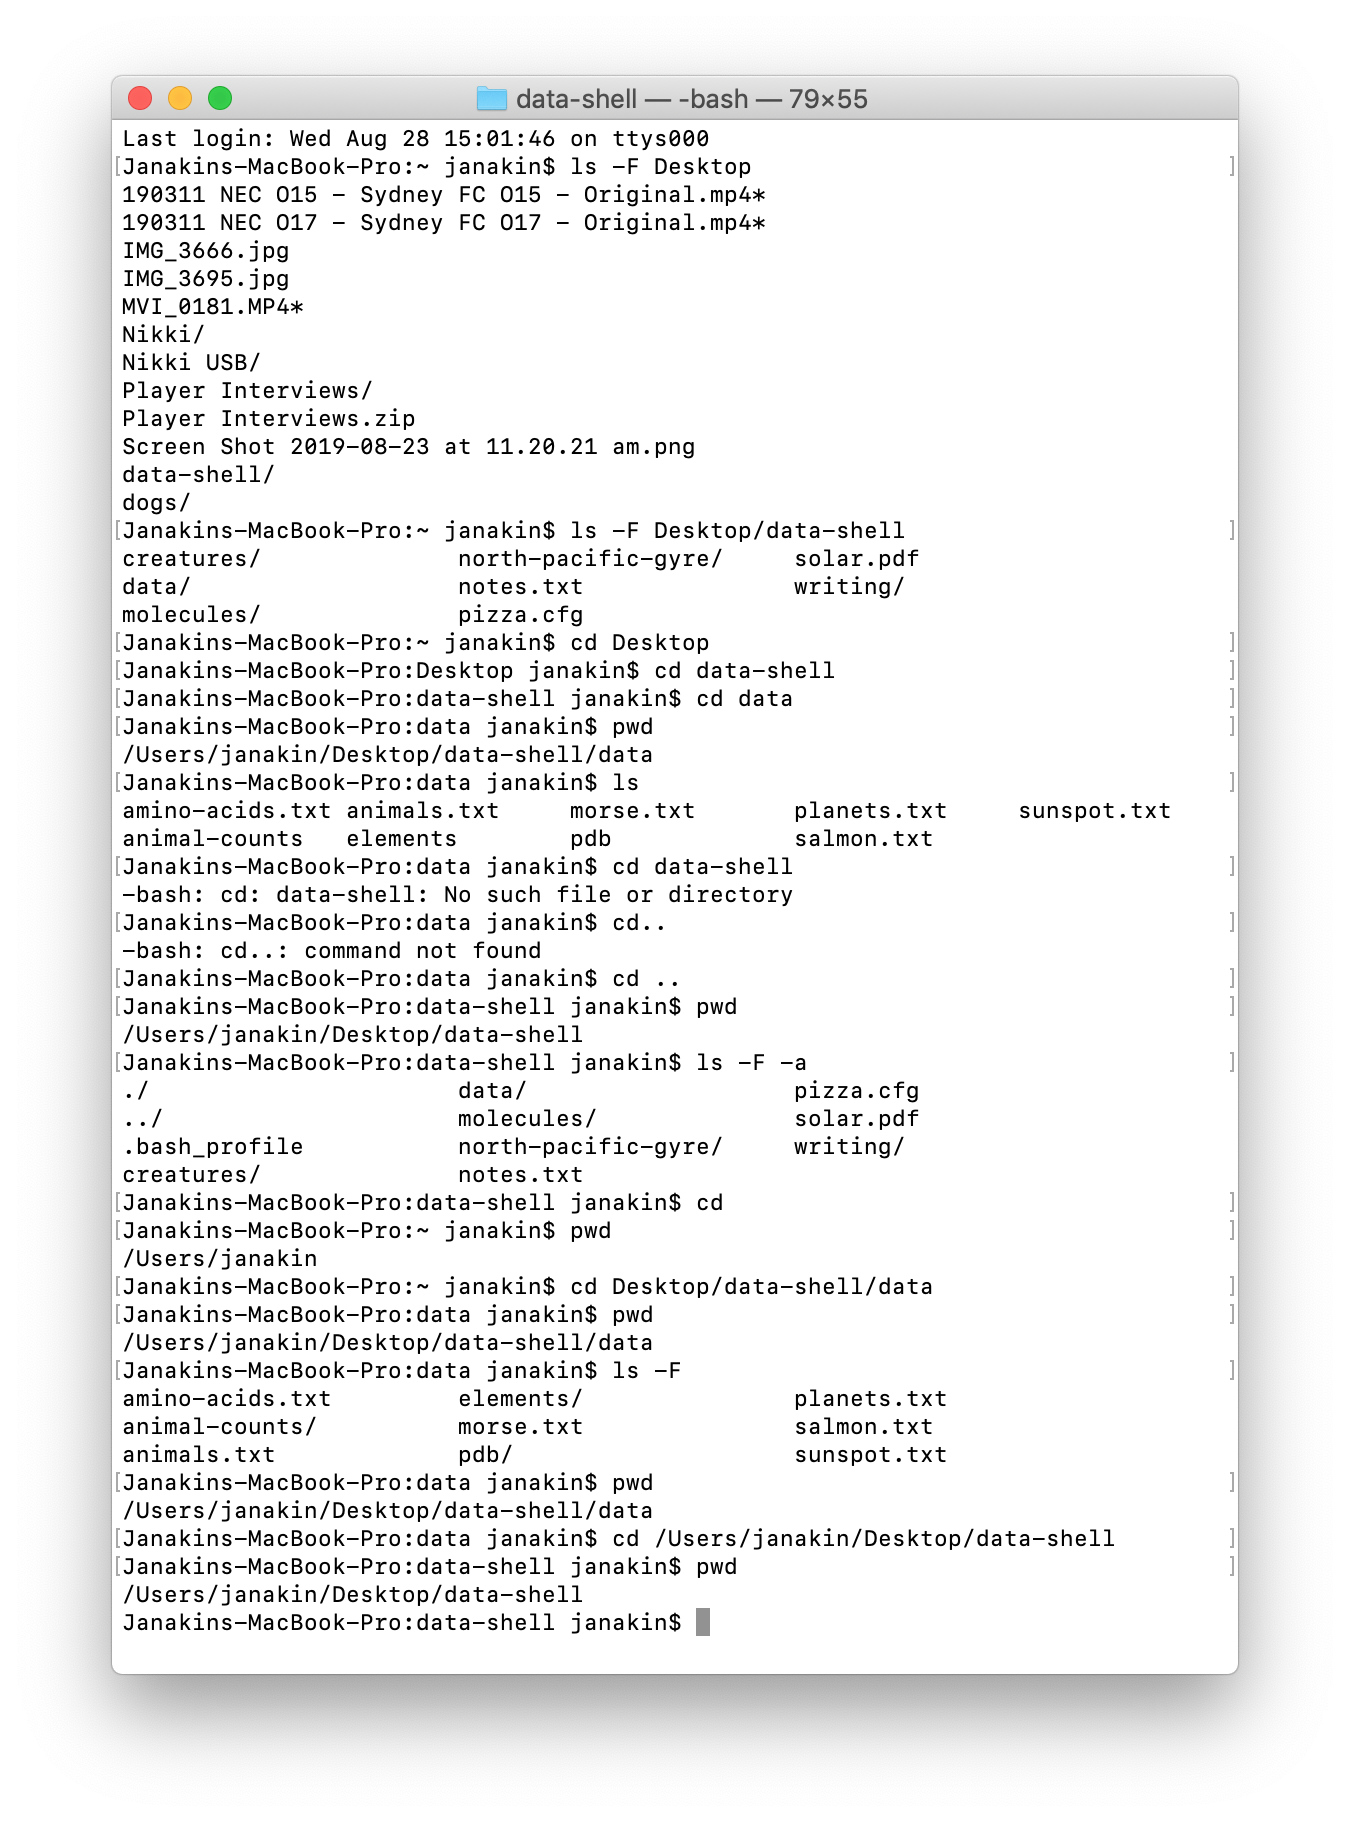
\includegraphics[width=\textwidth]{figc.png}

\section*{28/8/19 - 3:30pm}

Doing the exercise \textit{Absolute vs Relative Paths}

Amanda can only use these commands to navigate to the home directory.

\begin{verbatim}
    cd ~
    cd ~/data/..
    cd
    cd ..
\end{verbatim}

\section*{28/8/19 - 3:32pm}

Doing the exercise \textit{Relative Path Resolution}

If \begin{verbatim}
    pwd
\end{verbatim}
displays \begin{verbatim}
    /Users/thing
\end{verbatim}
 then \begin{verbatim}
     ls -F ../backup
 \end{verbatim} will display
 \begin{verbatim}
     original/ pnas_final/ pnas_sub/
 \end{verbatim}

\section*{28/8/19 - 3:35pm}

Doing the exercise \textit{ls Reading Comprehension}

The correct answer is 
\begin{verbatim}
    ls -r -F
    ls -r -F /Users/backup
\end{verbatim}

\section*{28/8/19 - 3:38pm}

Continuing with the lesson. Below is a screenshot of my Terminal progress.

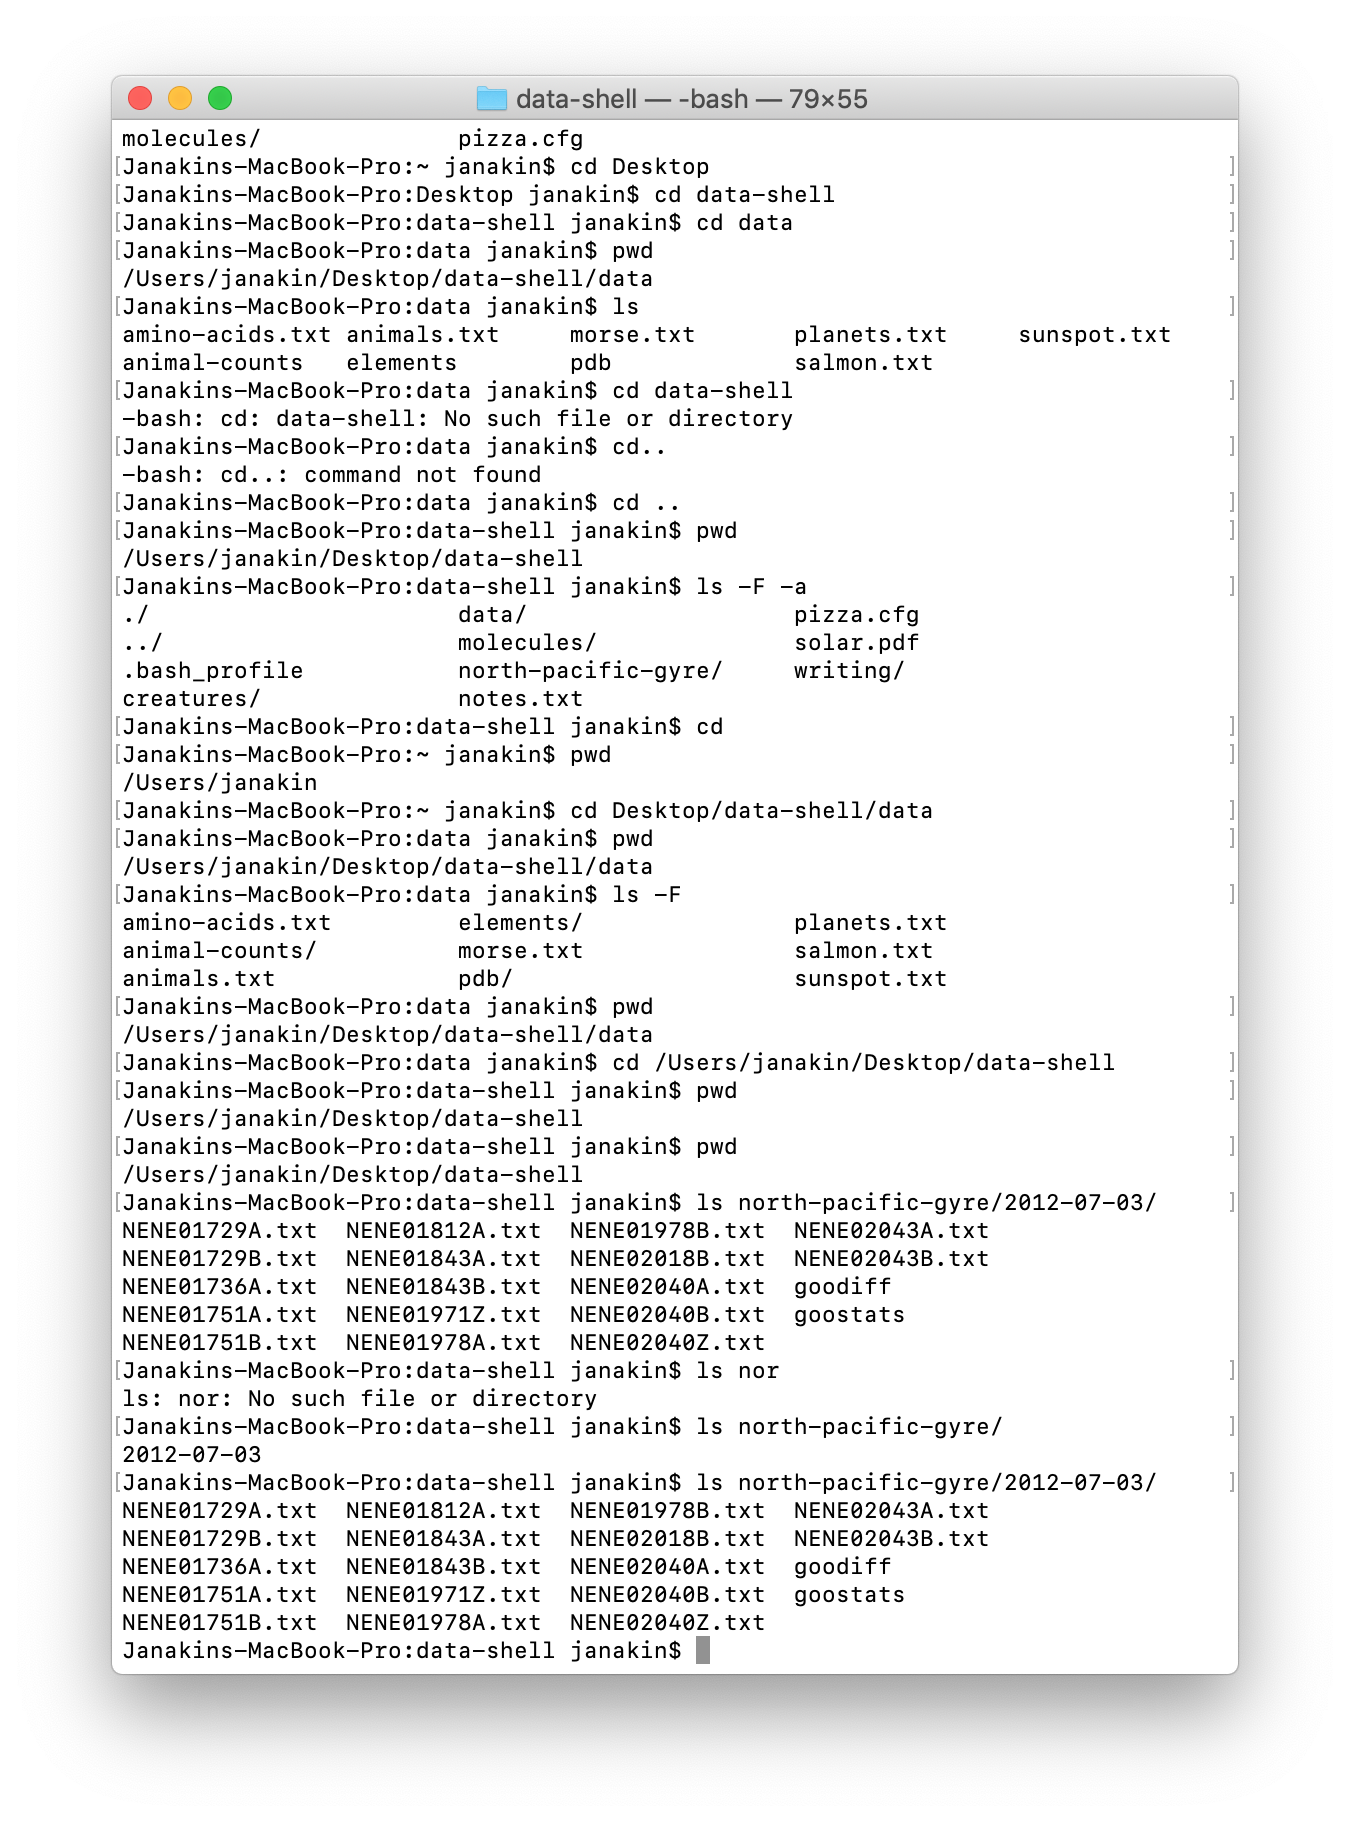
\includegraphics[width=\textwidth]{figd.png}

\section*{28/8/19 - 3:46pm}

Am now up to the next lesson \textbf{Working With Files and Directories}

\textbf{Objective:} Create a directory

\textbf{Action:} Entered command \begin{verbatim}
    mkdir thesis
\end{verbatim}

\textbf{Error:} None.

\textbf{Result:} New directory created.

\section*{28/8/19 - 3:47pm}

\textbf{Objective:} Create a text file.

\textbf{Action:}
\begin{itemize}
    \item Entered the commands \begin{verbatim}
        cd thesis
        nano draft.txt
    \end{verbatim}
    \item Entered text 'It's not "publish or perish anymore,
    it's "share and thrive".'
    \item Pressed Ctrl + O
    \item Pressed Enter
    \item Pressed Ctrl + X.
\end{itemize}

\textbf{Error:} None.

\textbf{Result:} New file draft.txt created.

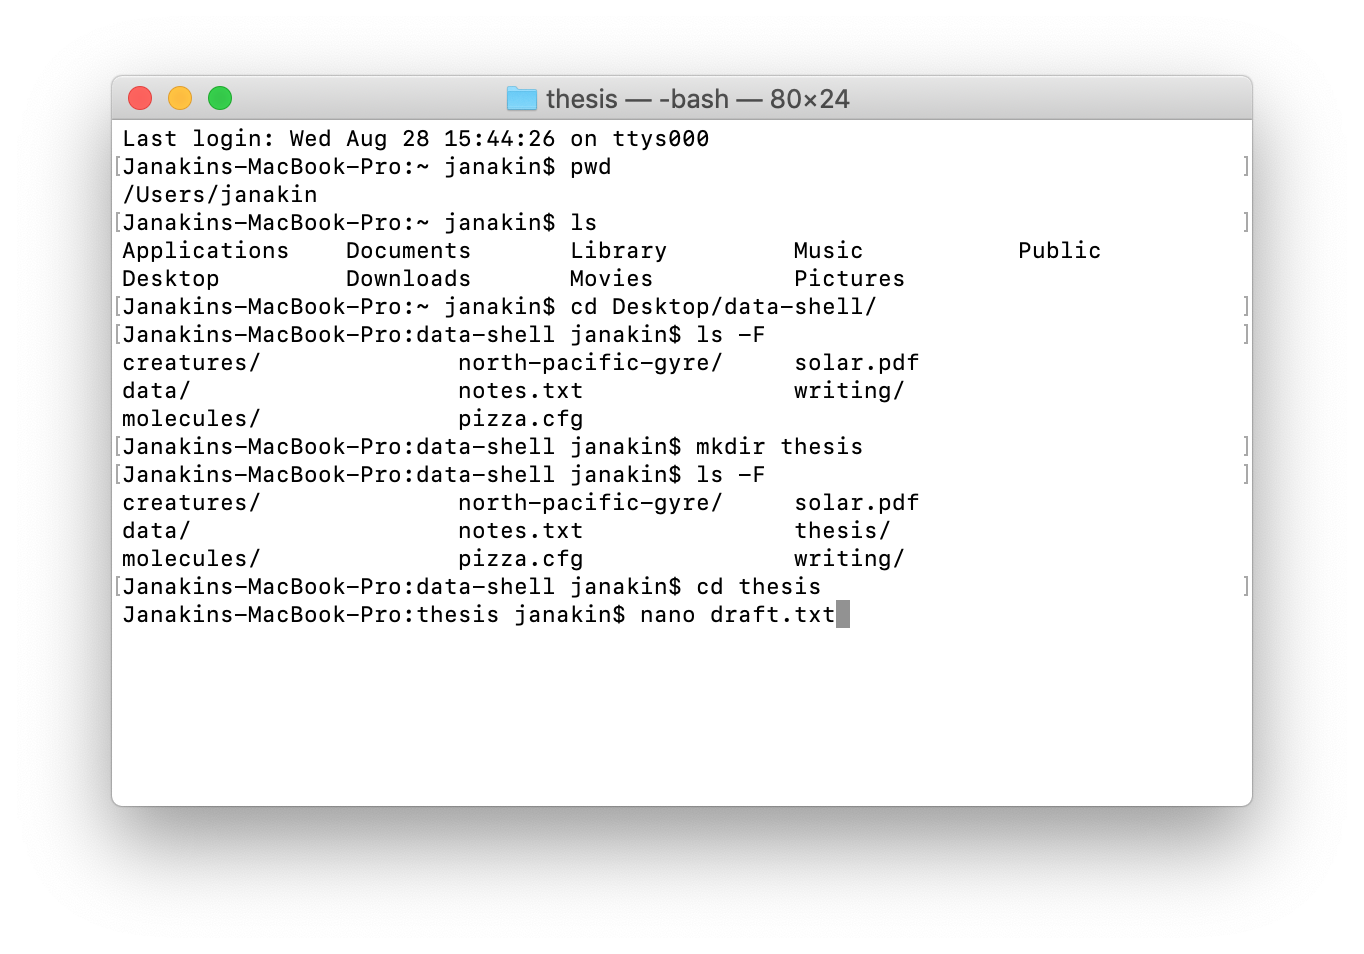
\includegraphics[width=\textwidth]{fige.png}

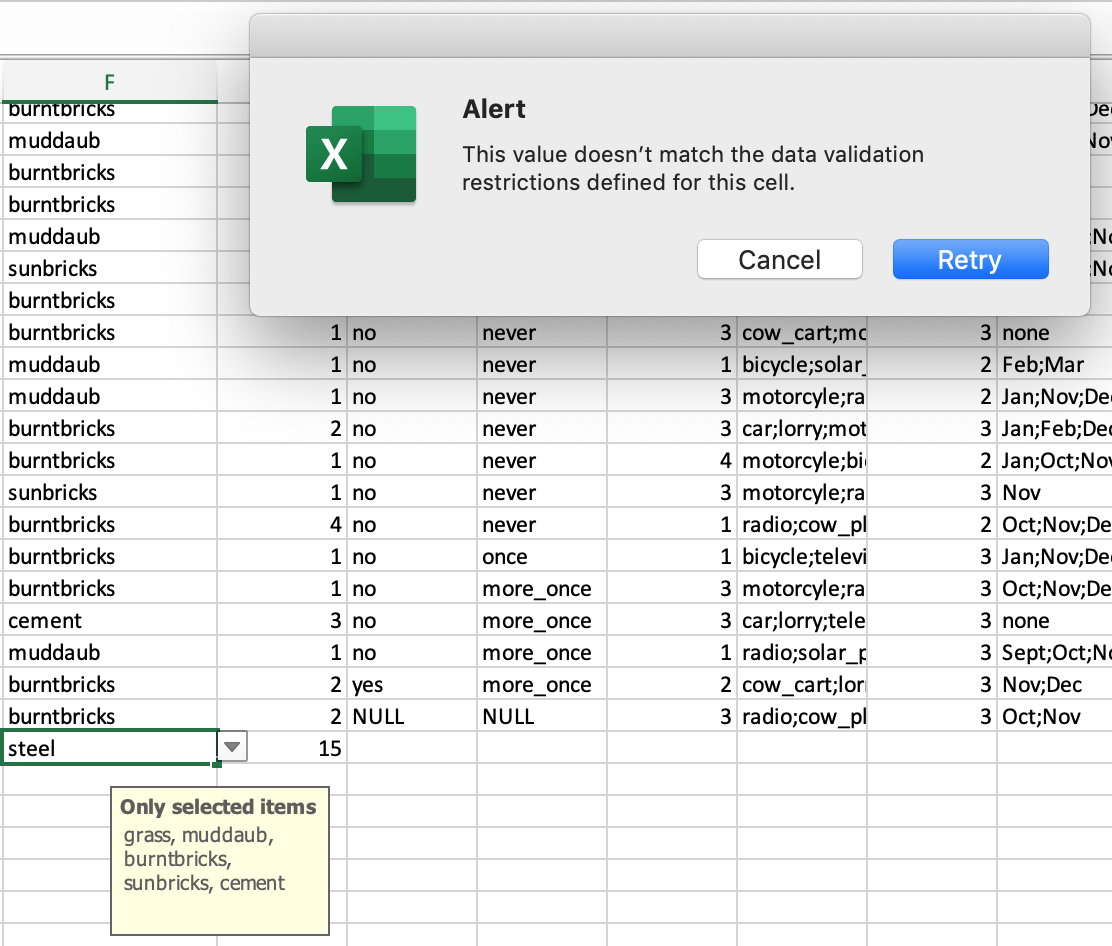
\includegraphics[width=\textwidth]{figf.png}

\section*{28/8/19 - 3:52pm}

\textbf{Objective:} Creating a file a different way.

\textbf{Action:} Entered the command \begin{verbatim}
    touch my_file.txt
\end{verbatim}

\textbf{Error:} None.

\textbf{Result:} New my\_file.txt created.

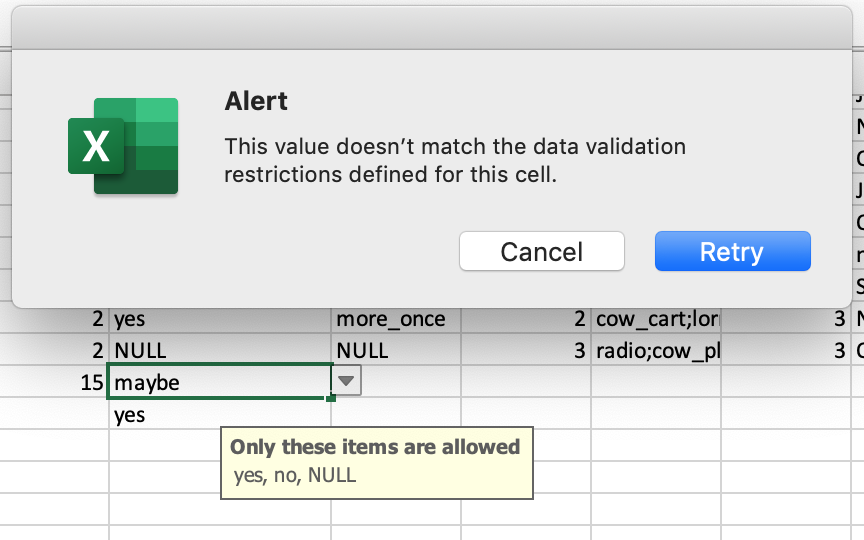
\includegraphics[width=\textwidth]{figg.png}

\section*{28/8/19 - 3:57pm}

\textbf{Objective:} Carry on with \textit{Moving files and directories} exercises.

\textbf{Action:} Entered the commands
\begin{verbatim}
    cd ~/Desktop/data-shell/
    mv thesis/draft.txt thesis/quotes.txt
    ls thesis
    mv thesis/quotes.txt .
    ls thesis
    ls quotes.txt
\end{verbatim}

\textbf{Error:} None.

\textbf{Result:} Success. Renamed and moved files as instructed from lesson.

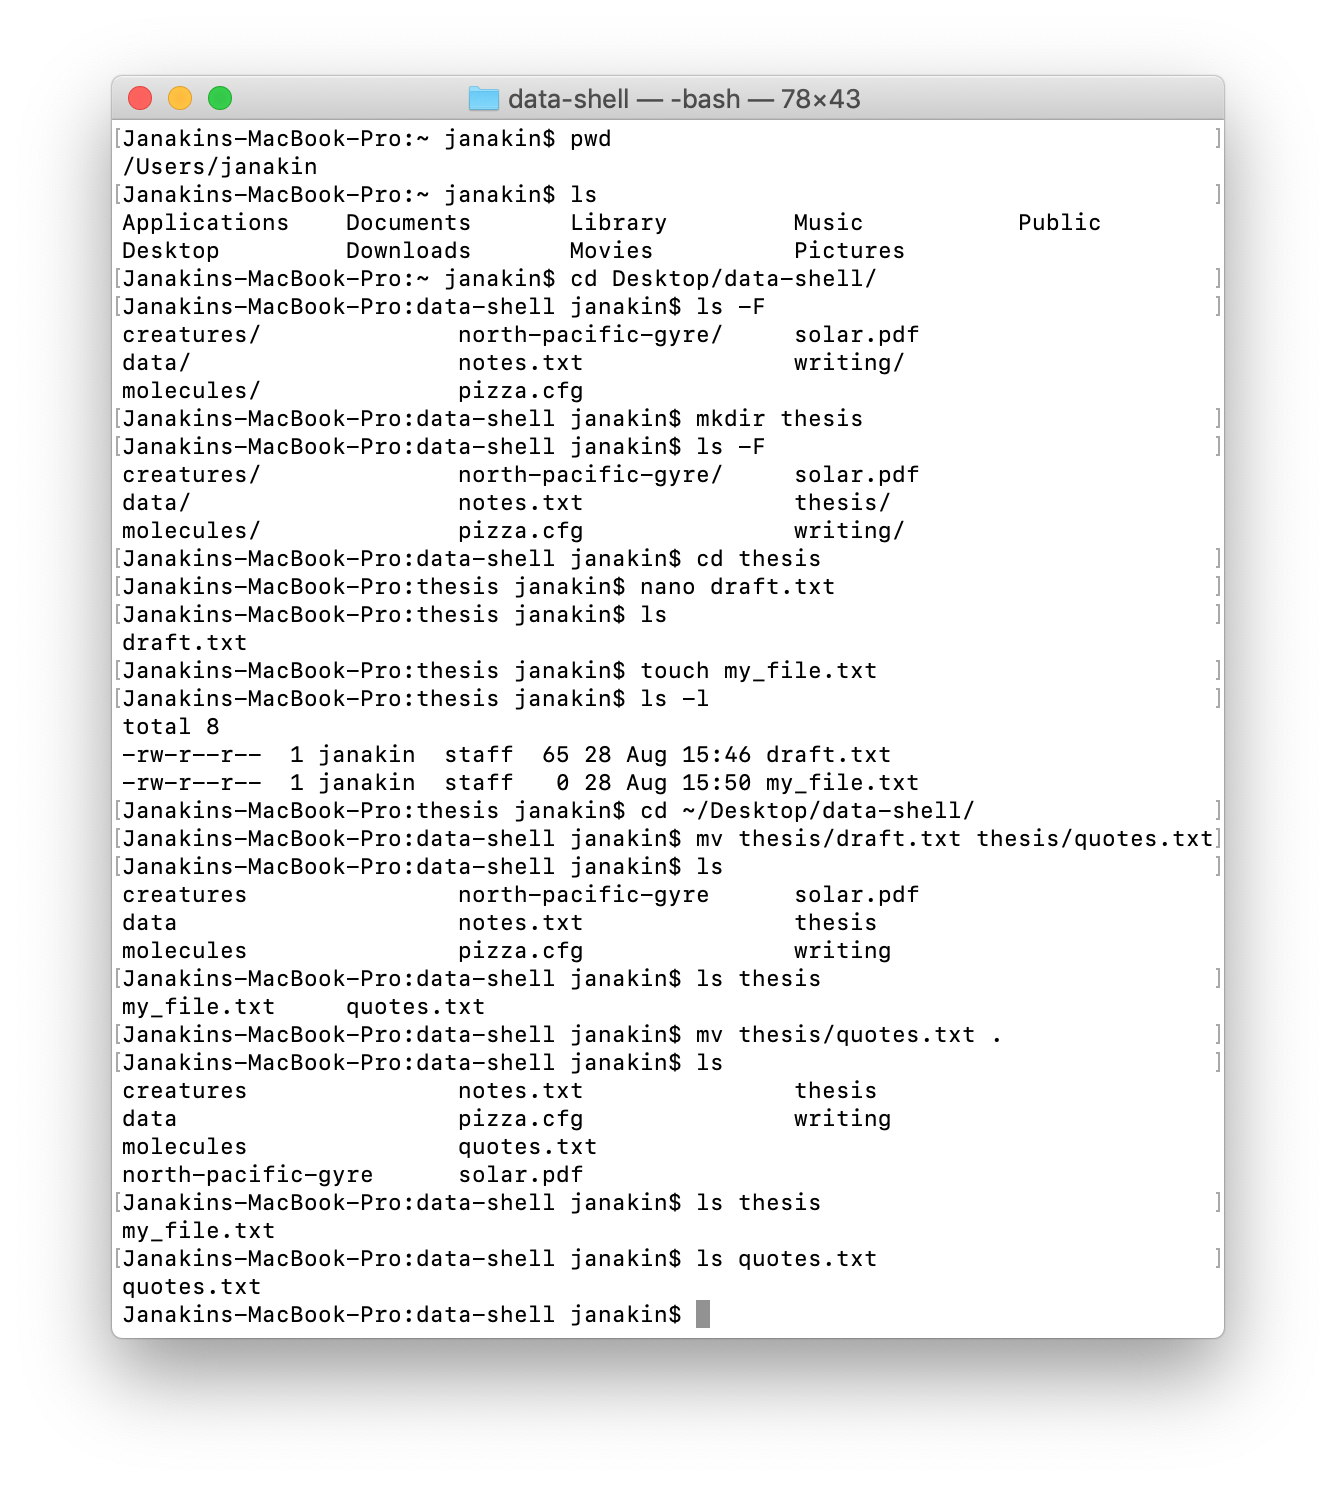
\includegraphics[width=\textwidth]{figh.png}

\section*{28/8/19 - 3:59pm}

Currently on exercise \textit{Moving to the Current Folder}. The correct command to move the files to the current folder is \begin{verbatim}
    mv ../analyzed/sucrose.dat ../analyzed/maltose.dat .
\end{verbatim}

\section*{28/8/19 - 4:02pm}

\textbf{Objective:} Copy files and directories.

\textbf{Action:} Entered the commands \begin{verbatim}
    cp quotes.txt thesis/quotations.txt
    ls quotes.txt thesis/quotations.txt
    cp -r thesis thesis_backup
    ls thesis thesis_backup
\end{verbatim}

\textbf{Error:} None.

\textbf{Result:} Successfully copied files and directories.

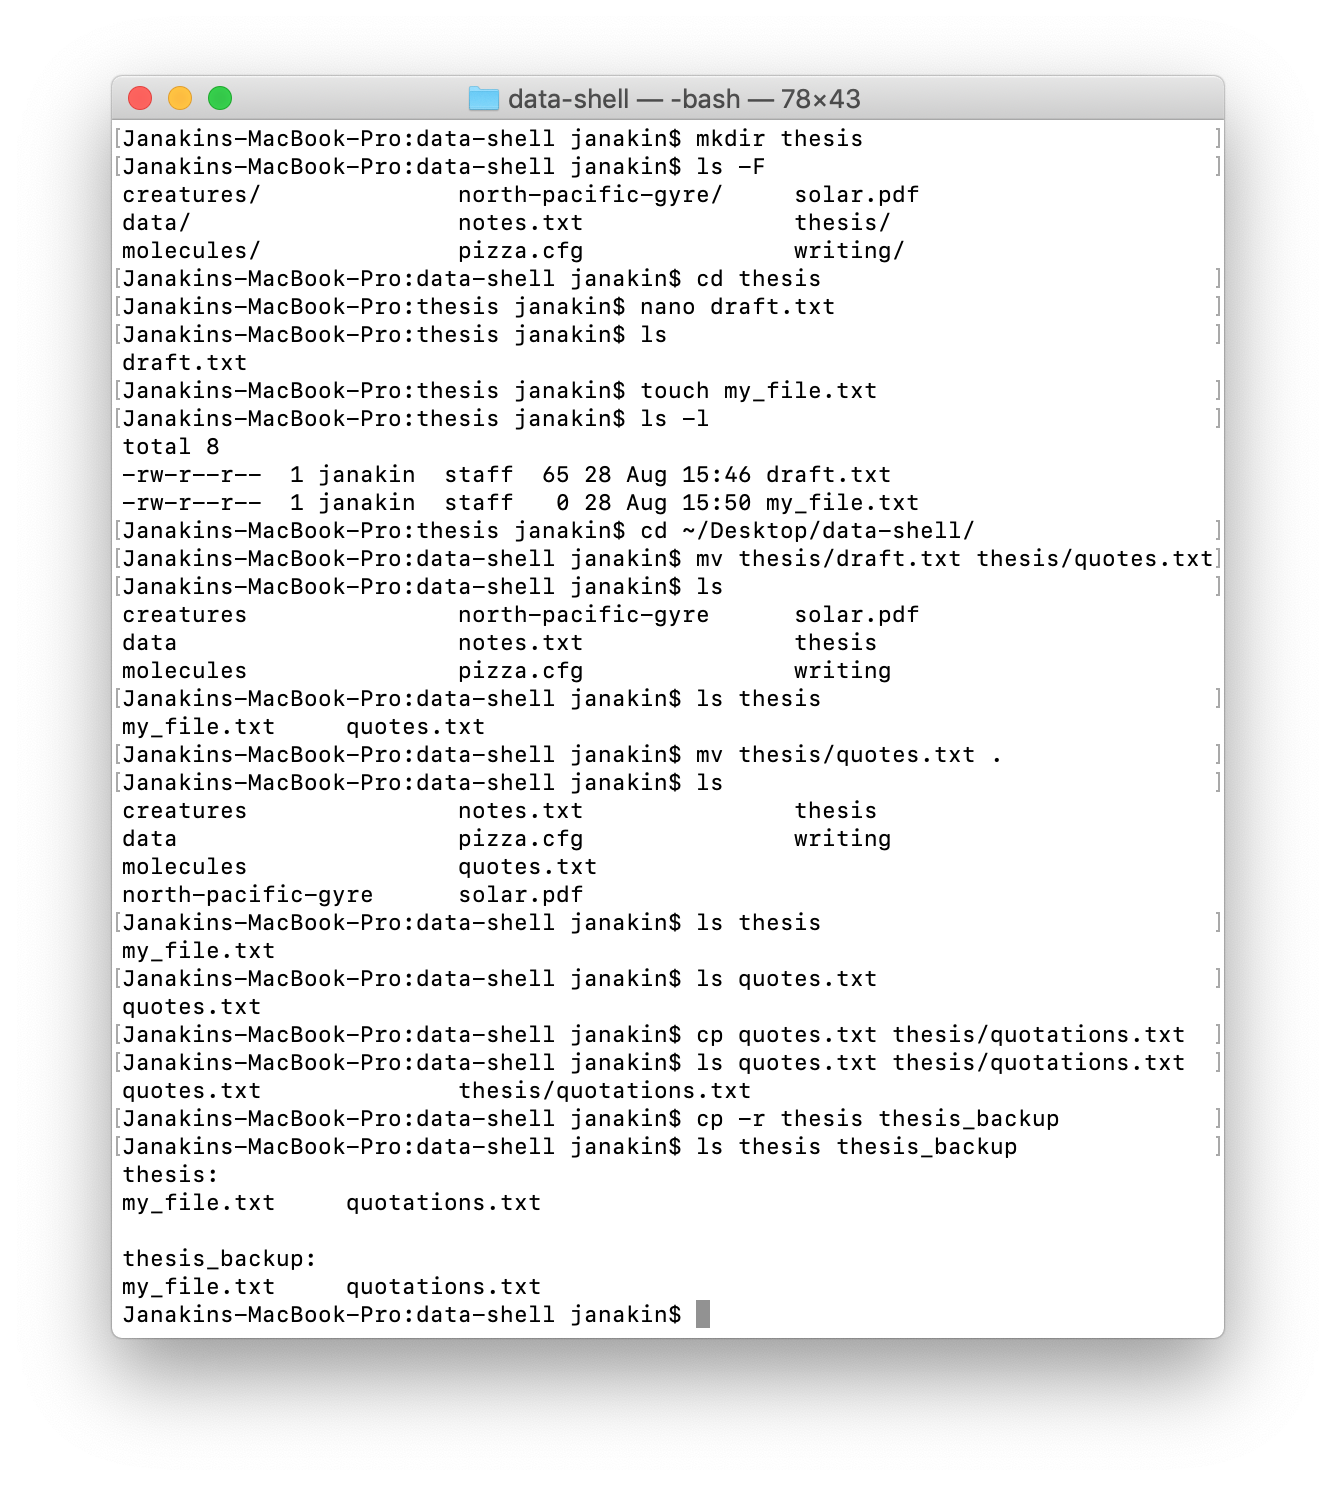
\includegraphics[width=\textwidth]{figi.png}

\section*{28/8/19 - 4:05pm}

On the exercise \textit{Renamimg files}. The command you would want to use is \begin{verbatim}
    mv statstics.txt statistics.txt
\end{verbatim}

\section*{28/8/19 - 4:07pm}

On the exercise \textit{Moving and copying}. The output is \begin{verbatim}
    recombine
\end{verbatim}

\section*{28/8/19 - 4:09pm}

\textbf{Objective:} Remove files and directories

\textbf{Action:} Entered the commands \begin{verbatim}
    rm quotes.txt
    ls quotes.txt
\end{verbatim}

\textbf{Error:} None.

\textbf{Result:} quotes.txt deleted.

\section*{28/8/19 - 4:10pm}

On the exercise \textit{Using rm Safely}. We would want to use \begin{verbatim}
    rm -i
\end{verbatim} to have Terminal confirm if we want to delete something. This is to ensure we don't accidently delete a file we did not intend to.

\section*{28/8/19 - 4:12pm}

\textbf{Objective:} Copy with Multiple Filenames

\textbf{Action:} Entered the commands \begin{verbatim}
    mkdir backup
    cp amino-acids.txt animals.txt backup/
    ls -F
    cp amino-acids.txt animals.txt morse.txt 
\end{verbatim}

\textbf{Error:} Unsure if an actual error or what the lesson wanted.

\textbf{Result:} See attached screen shot.

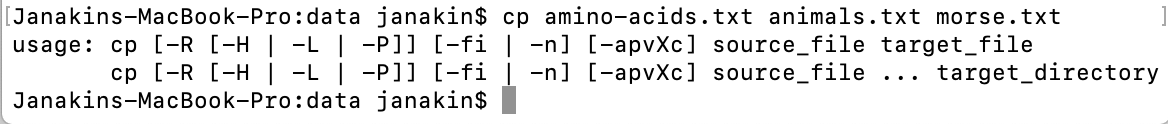
\includegraphics[width=\textwidth]{figj.png}

\section*{28/8/19 - 4:15pm}

On the exercise \textit{List filenames matching a pattern}. The answer is \#3.

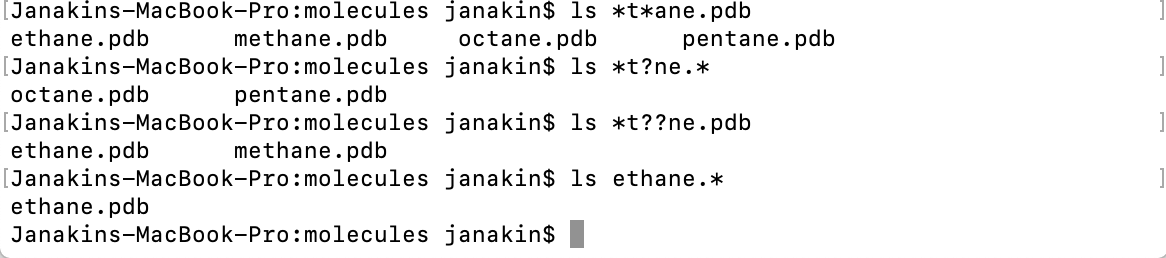
\includegraphics[width=\textwidth]{figk.png}

\section*{28/8/19 - 4:15pm}

On the exercise \textit{More on Wildcards}. The code I would enter is \begin{verbatim}
    cp *calibration.txt backup/calibration
    cp 2015-11-* send_to_bob/all_november_files/
    cp *-23-dataset* send_to_bob/all_datasets_created_on_a_23rd/
\end{verbatim}

\section*{28/8/19 - 4:15pm}

On the exercise \textit{Organizing Directories and Files}. The code I would enter is \begin{verbatim}
   mv *.dat analyzed
\end{verbatim}

\section*{28/8/19 - 4:17pm}

On the exercise \textit{Reproduce a folder structure}. The commands \begin{verbatim}
    mkdir 2016-05-20
    mkdir 2016-05-20/data
    mkdir 2016-05-20/data/processed
    mkdir 2016-05-20/data/raw
\end{verbatim}
and
\begin{verbatim}
    mkdir 2016-05-20
    cd 2016-05-20
    mkdir data
    cd data
    mkdir raw processed
\end{verbatim}

The third set of commands would produce an error because mkdir can't create a subdirectory in a non-existant one.

The final set of commands puts the 'raw' and 'processed' directories as the same level as the 'data' directory.

\end{document}
